%%%%%%%%%%%%%%%%%%%%%%%%%%%%%%%%%%%%%%%%%%%%%%%%%%%%%%%%%%%%%%%%%%%%%%%%%%%%%%%
\documentclass[hyperref={pdfpagelabels=false},compress,table]{beamer} % 在Mac下无法编译
% \documentclass[compress,table]{beamer} % 在Mac下使用
% package for font
\usepackage{fontspec}
\defaultfontfeatures{Mapping=tex-text}  %%如果没有它,会有一些 tex 特殊字符无法正常使用,比如连字符。
\usepackage{xunicode,xltxtra}
\usepackage[BoldFont,SlantFont,CJKnumber,CJKchecksingle]{xeCJK}  % \CJKnumber{12345}: 一万二千三百四十五
\usepackage{CJKfntef}  %%实现对汉字加点、下划线等。
\usepackage{pifont}  % \ding{}
% package for math
\usepackage{amsfonts}

% package for graphics
\usepackage[americaninductors,europeanresistors]{circuitikz}
\usepackage{tikz}
\usetikzlibrary{plotmarks}  % placements=positioning
\usepackage{graphicx}  % \includegraphics[]{}
\usepackage{subfigure}  %%图形或表格并排排列
% package for table
\usepackage{colortbl,dcolumn}  %% 彩色表格
\usepackage{multirow}
\usepackage{multicol}
\usepackage{booktabs}
% package for code
\usepackage{fancyvrb}
\usepackage{listings}

% \usepackage{animate}
% \usepackage{movie15}

%%%%%
% setting for beamer
\usetheme{default} % Madrid(常用), Copenhagen, AnnArbor, boxes(白色), Frankfurt,Berkeley
\useoutertheme[subsection=true]{miniframes} % 使用Berkeley时注释本行
\usecolortheme{sidebartab}
\usefonttheme{serif}  %%英文使用衬线字体
% \setbeamertemplate{background canvas}[vertical
% shading][bottom=white,top=structure.fg!7] %%背景色,上25%的蓝,过渡到下白。
\setbeamertemplate{theorems}[numbered]
\setbeamertemplate{navigation symbols}{}  %% 去掉页面下方默认的导航条
\setbeamercovered{transparent}  %设置 beamer 覆盖效果

% 设置标题title背景色
% \setbeamercolor{title}{fg=black, bg=lightgray!60!white}
\setbeamercolor{title}{fg=white, bg=black!70!white}

% 设置每页小LOGO
\pgfdeclareimage[width=1cm]{ouc}{figures/static/ouc.pdf}
\logo{\pgfuseimage{ouc}{\vspace{-20pt}}}

% setting for font
%%\setCJKmainfont{Adobe Kaiti Std}
\setCJKmainfont{SimSun} 
%% \setCJKmainfont{FangSong_GB2312} 
%% \setmainfont{Apple Garamond}  %%苹果字体没有SmallCaps
\setCJKmainfont{SimSun} 
%FUNNY%\setCJKmainfont{DFPShaoNvW5-GB}  %%华康少女文字W5(P)
%FUNNY%\setCJKmainfont{FZJingLeiS-R-GB}  %%方正静蕾体
%FUNNY%\setmainfont{Purisa}
%\setsansfont[Mapping=tex-text]{Adobe Song Std}
     %如果装了Adobe Acrobat,可在font.conf中配置Adobe字体的路径以使用其中文字体。
     %也可直接使用系统中的中文字体如SimSun、SimHei、微软雅黑等。
     %原来beamer用的字体是sans family;注意Mapping的大小写,不能写错。
     %设置字体时也可以直接用字体名,以下三种方式等同:
     %\setromanfont[BoldFont={黑体}]{宋体}
     %\setromanfont[BoldFont={SimHei}]{SimSun}
     %\setromanfont[BoldFont={"[simhei.ttf]"}]{"[simsun.ttc]"}
% setting for graphics
\graphicspath{{figures/}}  %%图片路径
\renewcommand\figurename{图}

% setting for pdf
\hypersetup{% pdfpagemode=FullScreen,%
            pdfauthor={Xiaodong Wang},%
            pdftitle={Title},%
            CJKbookmarks=true,%
            bookmarksnumbered=true,%
            bookmarksopen=false,%
            plainpages=false,%
            colorlinks=true,%
            citecolor=green,%
            filecolor=magenta,%
            linkcolor=blue,%red(default)
            urlcolor=cyan}

% setting for fontspec
\XeTeXlinebreaklocale "zh"  %%表示用中文的断行
\XeTeXlinebreakskip = 0pt plus 1pt minus 0.1pt  %%多一点调整的空间
%%%%%

% font setting by xeCJK
\setCJKfamilyfont{NSimSun}{NSimSun}
\newcommand{\song}{\CJKfamily{NSimSun}}
%%%\setCJKfamilyfont{AdobeSongStd}{Adobe Song Std}
%%%\newcommand{\AdobeSong}{\CJKfamily{AdobeSongStd}}
\setCJKfamilyfont{FangSong}{FangSong_GB2312}
\newcommand{\fang}{\CJKfamily{FangSong}}
%%%\setCJKfamilyfont{AdobeFangsongStd}{Adobe Fangsong Std}
%%%\newcommand{\AdobeFang}{\CJKfamily{AdobeFangsongStd}}
\setCJKfamilyfont{SimHei}{SimHei}
\newcommand{\hei}{\CJKfamily{SimHei}}
%%%\setCJKfamilyfont{AdobeHeitiStd}{Adobe Heiti Std}
%%%\newcommand{\AdobeHei}{\CJKfamily{AdobeHeitiStd}}
\setCJKfamilyfont{KaiTi}{KaiTi}
\newcommand{\kai}{\CJKfamily{KaiTi}}
%%%\setCJKfamilyfont{AdobeKaitiStd}{Adobe Kaiti Std}
\newcommand{\AdobeKai}{\CJKfamily{AdobeKaitiStd}}
\setCJKfamilyfont{LiSu}{LiSu}
\newcommand{\li}{\CJKfamily{LiSu}}
\setCJKfamilyfont{YouYuan}{YouYuan}
\newcommand{\you}{\CJKfamily{YouYuan}}
\setCJKfamilyfont{FZJingLei}{FZJingLeiS-R-GB}
\newcommand{\jinglei}{\CJKfamily{FZJingLei}}
\setCJKfamilyfont{MSYH}{Microsoft YaHei}
\newcommand{\msyh}{\CJKfamily{MSYH}}

% 自定义颜色
\def\Red{\color{red}}
\def\Green{\color{green}}
\def\Blue{\color{blue}}
\def\Mage{\color{magenta}}
\def\Cyan{\color{cyan}}
\def\Brown{\color{brown}}
\def\White{\color{white}}
\def\Black{\color{black}}

\lstnewenvironment{xmlCode}[1][]{% for Java
  \lstset{
    basicstyle=\tiny\ttfamily,%
    columns=flexible,%
    framexleftmargin=.7mm, %
    % frame=shadowbox,%
    % rulesepcolor=\color{cyan},%
     frame=single,%
    backgroundcolor=\color{white},%
    xleftmargin=4\fboxsep,%
    xrightmargin=4\fboxsep,%
    numbers=left,numberstyle=\tiny,%
    numberblanklines=false,numbersep=7pt,%
    language=xml, %
    }\lstset{#1}}{}

\lstnewenvironment{javaCode}[1][]{% for Java
  \lstset{
    basicstyle=\tiny\ttfamily,%
    columns=flexible,%
    framexleftmargin=.7mm, %
    frame=shadowbox,%
    rulesepcolor=\color{cyan},%
    % frame=single,%
    backgroundcolor=\color{white},%
    xleftmargin=4\fboxsep,%
    xrightmargin=4\fboxsep,%
    numbers=left,numberstyle=\tiny,%
    numberblanklines=false,numbersep=7pt,%
    language=Java, %
    }\lstset{#1}}{}

\lstnewenvironment{shCode}[1][]{% for Java
  \lstset{
    basicstyle=\scriptsize\ttfamily,%
    columns=flexible,%
    framexleftmargin=.7mm, %
    frame=shadowbox,%
    rulesepcolor=\color{brown},%
    % frame=single,%
    backgroundcolor=\color{white},%
    xleftmargin=4\fboxsep,%
    xrightmargin=4\fboxsep,%
    numbers=left,numberstyle=\tiny,%
    numberblanklines=false,numbersep=7pt,%
    language=sh, %
    }\lstset{#1}}{}

\newcommand\ask[1]{\vskip 4bp \tikz \node[rectangle,rounded corners,minimum size=6mm,
  fill=white,]{\Cyan \includegraphics[height=1.5cm]{question} \Large \msyh #1};}

\newcommand\wxd[1]{\vskip 4bp \tikz \node[rectangle,minimum size=6mm,
  fill=blue!60!white,]{\White \ding{118} \msyh #1};}

\newcommand\xyy[1]{\vskip 2bp \tikz \node[rectangle,minimum size=3mm,
  fill=black!80!white,]{\White \msyh\scriptsize #1};}

\newcommand\cxf[1]{\vskip 4bp \tikz \node[rectangle,rounded corners,minimum size=6mm,
  fill=orange!60!white,]{\White \ding{42} \msyh #1};}

\newcommand\samp[1]{\vskip 2bp \tikz \node[rectangle,minimum size=3mm,
  fill=white!100!white,]{\Mage\msyh \small CODE \ding{231} \Black #1};\vskip -8bp}

\newcommand\zhyfly[1]{\tikz \node[rectangle,rounded corners,minimum size=6mm,ball color=red!25!blue,text=white,]{#1};}

\setbeamerfont{frametitle}{series=\msyh} % 修改Beamer标题字体

\makeatletter
\newcommand{\Extend}[5]{\ext@arrow 0099{\arrowfill@#1#2#3}{#4}{#5}}
\makeatother


%%%%%%%%%%%%%%%%%%%%%%%%%%%%%%%%%%%%%%%%%%%%%%%%%%%%%%%%%%%%%%%%%%%%%%%%%%%%%%%
% \titlepage
\title[Wang Xiaodong]{\hei {\huge Java 应用与开发}\\  
  Java数组和字符串}
\author[王晓东]{王晓东\\
  \href{mailto:wangxiaodong@ouc.edu.cn}{\footnotesize wangxiaodong@ouc.edu.cn}}
\institute[中国海洋大学]{\small 中国海洋大学}
\date{\today}
\titlegraphic{\vspace{-6em}
\includegraphics[height=6cm]{static/ouc.pdf}\vspace{-6em}}
%%%%%%%%%%%%%%%%%%%%%%%%%%%%%%%%%%%%%%%%%%%%%%%%%%%%%%%%%%%%%%%%%%%%%%%%%%%%%%%
\begin{document}
%% Delete this, if you do not want the table of contents to pop up at
%% the beginning of each subsection:
\AtBeginSection[]{                              % 在每个Section前都会加入的Frame
  \frame<handout:0>{
    \frametitle{\textbf{\hei 接下来…}}
    \tableofcontents[currentsection]
  }
}  %

\AtBeginSubsection[]                            % 在每个子段落之前
{
  \frame<handout:0>                             % handout:0 表示只在手稿中出现
  {
    \frametitle{\textit{\hei 接下来…}}\small
    \tableofcontents[current,currentsubsection] % 显示在目录中加亮的当前章节
  }
}
 \frame{\titlepage}

%%%%%%%%%%%%%%%%%%%%%%%%%%%%%%%%%%%%%%%%%%%%%%%%
\begin{frame}
\frametitle{参考书目}
\begin{enumerate}
\item 陈国君等编著, Java程序设计基础(第5版), 清华大学出版社
\item Bruce Eckel, Thinking in Java (3rd)
\end{enumerate}  
\end{frame}

\begin{frame}
  \frametitle{学习目标}
  \begin{enumerate}
  \item 掌握Java数组的概念
  \item 学会一维数组和二维数组的使用;认识Arrays类,掌握操作数组相关方法
  \item 掌握Java字符串的概念,字符串与数组的关系;学会String类常用字符串操作方法
  \end{enumerate}
\end{frame}

\section*{大纲}
\frame{\frametitle{大纲} \tableofcontents }

\section{数组的概念}

\begin{frame}[fragile] % [fragile]参数使得能够插入代码
  \frametitle{数组的基本概念}

  {\hei 数组是相同数据类型的元素按一定顺序排列的集合。}Java中,数组元素既可以为基本数据类型,也可以为对象。

  \wxd{Java的内存分配(基础)}
  
  \begin{description}
  \item [栈内存] 存放定义的基本类型的变量和对象的引用变量,超出作用域将自动释放。
  \item [堆内存] 存放由new运算符创建的对象和数组,由Java虚拟机的自动垃圾回收器来管理。
  \end{description}
\end{frame}

\begin{frame}[fragile]
  \frametitle{数组的主要特点}
  \begin{itemize}
  \item 数组是相同数据类型的元素的集合;
  \item 数组中的各元素有先后顺序,它们在内存中按照这个先后顺序连续存放;
  \item 数组的元素用整个数组的名字和它自己在数组中的顺序位置来表示。
  \end{itemize}

  {\Blue\kai 例如,a[0]表示名字为a的数组中的第一个元素,a[1]表示数组a的第二个元素,依次类推。}

\end{frame}

\section{一维数组}

\begin{frame}[fragile]
  \frametitle{一维数组}

  创建Java数组一般需经过三个步骤:

  \begin{enumerate}
  \item 声明数组
  \item 创建内存空间
  \item 创建数组元素并赋值
  \end{enumerate}
  
  \samp{一维数组创建声明和内存分配}
  
  \begin{javaCode}
    int[] x;  //声明名称为x的int型数组,未分配内存给数组
    x = new int[10];   //x中包含有10个元素,并分配空间
  \end{javaCode}

  \begin{javaCode}
    int[] x = new int[10];   //声明数组并动态分配内存
  \end{javaCode}

\xyy{动态内存分配说明}

{\kai 用new分配内存的同时,数组的每个元素都会自动赋默认值,整型为0,实数为0.0,布尔型为false,引用型为null。}

\end{frame}

\begin{frame}[fragile]
  \frametitle{一维数组}

  \wxd{一维数组的初始化}

  若在声明数组时进行赋值即初始化称为静态内存分配。

  \rule[0pt]{10cm}{0.05em}
  
  {\kai 数据类型[] 数组名={初值0,初值1,…,初值n};}
  
  \rule[0pt]{10cm}{0.05em}
  
  \samp{一维数组静态初始化}

  \begin{javaCode}
    int[]  a = {1,2,3,4,5};
  \end{javaCode}

\cxf{注意}

在Java程序中声明数组时,无论用何种方式定义数组,都不能指定其长度。

\codeset{sample.array.ArraySample.java}
\end{frame}

\section{二维数组}

\begin{frame}[fragile]
  \frametitle{二维数组}

  Java中无真正的多维数组,只是数组的数组。

  \wxd{二维数组的声明和内存分配}

  \rule[0pt]{10cm}{0.05em}

  {\kai 数据类型[] [] 数组名;\\
  数组名 = new 数据类型 [行数] [列数];\\
  数据类型[] [] 数组名 = new 数据类型 [行数][列数];
  }
  
  \rule[0pt]{10cm}{0.05em}

  \begin{figure}
    \centering
    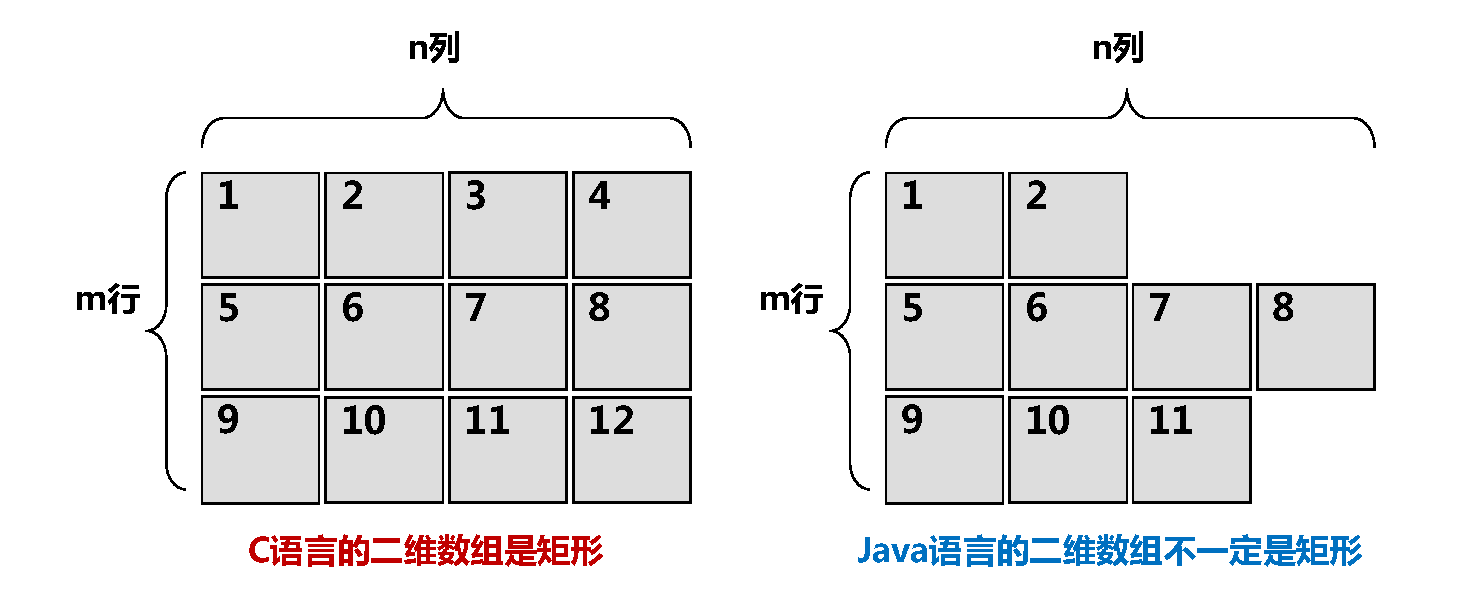
\includegraphics[width=.8\textwidth]{ppt/2-dim-array.pdf}
  \end{figure}
\end{frame}

\begin{frame}[fragile]
  \frametitle{二维数组定义的含义}
  \begin{itemize}[<+-| structure@+>]
  \item Java中的二维数组看作是由多个一维数组构成
  \item 二维数组申请内存必须指定{\Red 高层维数}\\
    \fbox{int[][] myArray1 = new int[10][];}\\
    \fbox{int[][] myArray2 = new int[10][3];}
  \item \fbox{int[][] x;}\\
    {\kai\Blue 表示定义了一个数组引用变量x,第一个元素为x[0],最后一个为x[n-1],其长度不确定}
  \item \fbox{x = new int[3][];}\\
    {\kai\Blue 表示数组x有三个元素,每个元素都是int[]类型的一维数组,分别为int x[0][]、int[] x[1]、int[] x[2]}\\
    \fbox{x[0] = new int[3];  x[1] = new int[2];}\\
    {\kai\Blue 给x[0]、x[1]、x[2]赋值(长度可以不一样)}
  \end{itemize}
\end{frame}

\begin{frame}[fragile]
  \frametitle{二维数组赋初值}

  \begin{javaCode}
    int[][] a = {{11,22,33,44}, {66,77,88,99}};    
  \end{javaCode}

  \cxf{注意}

  声明多维数组并初始化时不能指定其长度,否则出错。

  \codeset{sample.array.Array2DimSample.java}

\end{frame}

\begin{frame}[fragile]
  \frametitle{Arrays类}

  java.util.Arrays工具类能方便地操作数组,它提供的所有方法都是静态的。该类具有以下功能:

  \begin{description}
  \item[给数组赋值] 通过fill方法。
  \item[对数组排序] 通过sort方法。
  \item[比较数组] 通过equals方法比较数组中元素值是否相等。
  \item[查找数组元素] 通过binarySearch方法能对排序好的数组进行二分查找法操作。
  \item[复制数组] 把数组复制成一个长度为length的新数组。
  \end{description}

  \codeset{sample.array.ArrayToolsSample.java}
\end{frame}

\section{字符串}

\begin{frame}[fragile]
  \frametitle{字符串变量的创建}

  字符串是用一对双引号括起来的字符序列。Java语言中,字符串常量或变量均用类实现。

  \wxd{字符串变量的创建}

  \samp{格式1}
  \begin{javaCode}
    String s;                  //声明字符串型引用变量s,此时s的值为null
    s = new String("Hello");   //在堆内存中分配空间,并将s指向该字符串首地址 
  \end{javaCode}

  \samp{格式2}
  \begin{javaCode}
    String s = new String("Hello");
  \end{javaCode}

  \samp{格式3}
  \begin{javaCode}
    String s = "Hello";
  \end{javaCode}

\end{frame}

\begin{frame}[fragile]
  \frametitle{String类的常用方法}

  \samp{求字符串长度}

  \begin{javaCode}
    String str = new String("asdfzxc");
    int strlength = str.length(); //strlength = 7
  \end{javaCode}

  \samp{获取字符串某一位置字符}

  \begin{javaCode}
    char ch = str.charAt(4); //ch = z
  \end{javaCode}

  \samp{提取子串}

  \begin{javaCode}
    String str2 = str1.substring(2); //str2 = "dfzxc"
    String str3 = str1.substring(2,5); //str3 = "dfz"
  \end{javaCode}

  \samp{字符串连接}

  \begin{javaCode}
    String str = "aa".concat("bb").concat("cc");
    String str = "aa" + "bb" + "cc"; // 相当于上一行
  \end{javaCode}

\end{frame}

\begin{frame}[fragile]
  \frametitle{String类的常用方法}

  \samp{字符串比较}

  \begin{javaCode}
    String str1 = new String("abc");
    String str2 = new String("ABC");
    int a = str1.compareTo(str2);  //a>0
    int b = str1.compareTo(str2);  //b=0
    boolean c = str1.equals(str2); //c=false
    boolean d = str1.equalsIgnoreCase(str2); //d=true
  \end{javaCode}

  \samp{字符串中字符的大小写转换}

  \begin{javaCode}
    String str = new String("asDF");
    String str1 = str.toLowerCase(); //str1 = "asdf"
    String str2 = str.toUpperCase(); //str2 = "ASDF"
  \end{javaCode}

  \samp{字符串中字符的替换}

  \begin{javaCode}
    String str = "asdzxcasd";
    String str1 = str.replace('a','g'); //str1 = "gsdzxcgsd"
    String str2 = str.replace("asd","fgh"); //str2 = "fghzxcfgh"
    String str3 = str.replaceFirst("asd","fgh"); //str3 = "fghzxcasd"
    String str4 = str.replaceAll("asd","fgh"); //str4 = "fghzxcfgh"
  \end{javaCode}

\homework{请自行总结常用的字符串操作方法。}
\end{frame}

\begin{frame}[fragile]
  \frametitle{理解Java字符串}

  \samp{String.java Part 1}
  \begin{javaCode}
    public final class String
    implements java.io.Serializable, Comparable<String>, CharSequence { //1
    /** The value is used for character storage. */
    private final char value[]; //2

    /** The offset is the first index of the storage that is used. */
    private final int offset;

    /** The count is the number of characters in the String. */
    private final int count;

    /** Cache the hash code for the string */
    private int hash; // Default to 0

    /** use serialVersionUID from JDK 1.0.2 for interoperability */
    private static final long serialVersionUID = -6849794470754667710L;
    ........
}
  \end{javaCode}

  \begin{enumerate}\kai\small
  \item String类是final类,即意味着String类不能被继承,并且它的成员方法都默认为final方法。
  \item 从String类的成员属性可以看出String类其实是通过char数组来保存字符串的。
  \end{enumerate}
\end{frame}


\begin{frame}[fragile]
  \frametitle{理解Java字符串}

  \samp{String.java Part 2}
  \begin{javaCode}
    public String substring(int beginIndex, int endIndex) {
      if (beginIndex < 0) {
        throw new StringIndexOutOfBoundsException(beginIndex);
      }
      if (endIndex > count) {
        throw new StringIndexOutOfBoundsException(endIndex);
      }
      if (beginIndex > endIndex) {
        throw new StringIndexOutOfBoundsException(endIndex - beginIndex);
      }
      return ((beginIndex == 0) && (endIndex == count)) ? this :
      new String(offset + beginIndex, endIndex - beginIndex, value);
    }
  \end{javaCode}

  \begin{enumerate}\kai\small
  \item 无论是substring还是concat操作等都不是在原有的字符串上进行的,而是重新生成了一个新的字符串对象,最原始的字符串并没有被改变。
  \item {\hei\Red String对象一旦被创建就是固定不变的,对String对象的任何操作都不影响到原对象,而是会生成新的对象。}
  \end{enumerate}
\end{frame}

\begin{frame}
  \frametitle{本节习题}

  \wxd{小编程}
  \begin{enumerate}
  \item 编写程序,求一个三阶方阵的对角线上各元素之和。
  \item 编写程序,从键盘上输入一个字符串和子串开始位置与长度,截取该字符串的子串并输出。
  \item 编写程序,统计用户从键盘输入的字符串中包含的字母、数字和其他字符的个数。
  \end{enumerate}
\end{frame}

%%%%%%%%%%%%%%%%%%%%%%%%%%%%%%%%%%%%%%%%%%%%%%%%%%%%%%%%%%%%%%%%%%%%%%%%%%%%%%%
% TKS Page %%%%%%%%%%%%%%%%%%%%%%%%%%%%%%%%%%%%%%%%%%%%
\begin{frame}
\centering
{\Huge \textcolor{blue}{THE END}} \\
\vspace{5mm}
{\Large wangxiaodong@ouc.edu.cn} \\
\end{frame}
%%%%%%%%%%%%%%%%%%%%%%%%%%%%%%%%%%%%%%%%%%%%%%%%%%%%%%%
%%%%%%%%%%%%%%%%%%%%%%%%%%%%%%%%%%%%%%%%%%%%%%%%%%%%%%%%%%%%%%%%%%%%%%%%%%%%%%%
\end{document}
